\hypertarget{interface_t_p_chart_o_meter}{
\section{TPChartOMeter Class Reference}
\label{interface_t_p_chart_o_meter}\index{TPChartOMeter@{TPChartOMeter}}
}
{\tt \#import $<$TPChartOMeter.h$>$}

Inheritance diagram for TPChartOMeter::\begin{figure}[H]
\begin{center}
\leavevmode
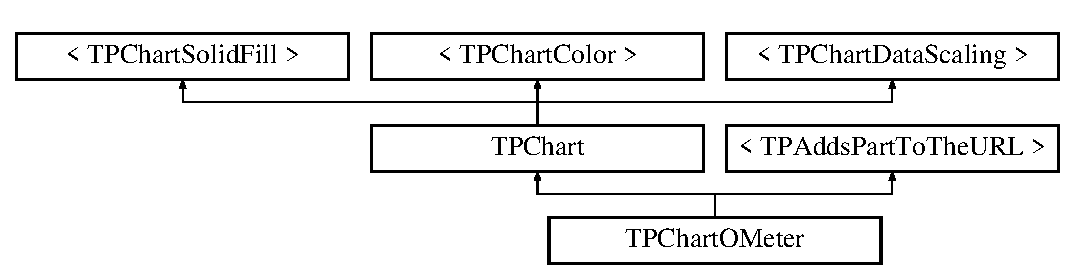
\includegraphics[height=3cm]{interface_t_p_chart_o_meter}
\end{center}
\end{figure}
\subsection*{Properties}
\begin{CompactItemize}
\item 
int \hyperlink{interface_t_p_chart_o_meter_f28c79861d8123f6294791942243c0aa}{value}
\item 
NSString $\ast$ \hyperlink{interface_t_p_chart_o_meter_13fa16f1efed823bb7dc221355688312}{label}
\end{CompactItemize}


\subsection{Detailed Description}
Google-o-meter diagram\par
 example: \href{http://chart.apis.google.com/chart?chs=225x125&cht=gom&chd=t:70&chl=Hello}{\tt http://chart.apis.google.com/chart?chs=225x125\&cht=gom\&chd=t:70\&chl=Hello} 

\subsection{Property Documentation}
\hypertarget{interface_t_p_chart_o_meter_13fa16f1efed823bb7dc221355688312}{
\index{TPChartOMeter@{TPChartOMeter}!label@{label}}
\index{label@{label}!TPChartOMeter@{TPChartOMeter}}
\subsubsection[{label}]{\setlength{\rightskip}{0pt plus 5cm}- (NSString $\ast$) label\hspace{0.3cm}{\tt  \mbox{[}read, write, retain\mbox{]}}}}
\label{interface_t_p_chart_o_meter_13fa16f1efed823bb7dc221355688312}


A label for the arrow \hypertarget{interface_t_p_chart_o_meter_f28c79861d8123f6294791942243c0aa}{
\index{TPChartOMeter@{TPChartOMeter}!value@{value}}
\index{value@{value}!TPChartOMeter@{TPChartOMeter}}
\subsubsection[{value}]{\setlength{\rightskip}{0pt plus 5cm}- (int) value\hspace{0.3cm}{\tt  \mbox{[}read, write, assign\mbox{]}}}}
\label{interface_t_p_chart_o_meter_f28c79861d8123f6294791942243c0aa}


The value to display\par
 range: 0-100 

The documentation for this class was generated from the following file:\begin{CompactItemize}
\item 
TPChartOMeter.h\end{CompactItemize}
